\documentclass{beamer}
\usetheme{Madrid}
\usecolortheme{default}
\usepackage{tikz}

\title{Arguments from Authority}
\subtitle{Why We Trust and When We Shouldn't}
\author{Brendan Shea, PhD}
\date{Intro to Logic}

\begin{document}
	
	% Slide 1: Title Slide
	\frame{\titlepage}
	
	% Slide 2: Arguments from Authority: Why We Trust and When We Shouldn't
	\begin{frame}
		\frametitle{Arguments from Authority: Why We Trust and When We Shouldn't}
		\begin{itemize}
			\item An \textbf{argument from authority} (or \textbf{appeal to authority}) occurs when we accept a claim because an expert or authority figure says it's true.
			\item We encounter these arguments daily: your doctor prescribes medication, a mechanic diagnoses your car, or a professor explains quantum physics.
			\item While often necessary and reasonable, appeals to authority can lead us astray when misused or when we trust the wrong sources.
			\item This lecture explores how to distinguish legitimate appeals to authority from fallacious ones, using medical examples throughout history.
		\end{itemize}
		
		\begin{alertblock}{Key Question}
			How do we decide which authorities deserve our trust?
		\end{alertblock}
	\end{frame}
	
	% Slide 3: Course Overview: Medical Examples and Beyond
	\begin{frame}
		\frametitle{Overview: Medical Examples and Beyond}
		\begin{itemize}
			\item We'll examine how medical authorities have both helped and harmed throughout history, from ancient bloodletting to modern social media health influencers.
			\item You'll learn to identify the structure of arguments from authority and recognize when they're being used appropriately versus misleadingly.
			\item We'll develop practical tools for evaluating experts, understanding scientific consensus, and navigating conflicting opinions.
			\item By the end, you'll have a framework for balancing necessary trust in experts with healthy skepticism.
		\end{itemize}
		
		\begin{example}
			Consider: Why do you believe smoking causes cancer? Most of us haven't conducted the research ourselves—we trust medical authorities.
		\end{example}
	\end{frame}
	
	% Slide 4: What Is an Argument from Authority?
	\begin{frame}
		\frametitle{What Is an Argument from Authority?}
		\begin{itemize}
			\item An \textbf{argument from authority} has the basic structure: "X is true because authority A says X is true."
			\item This is an \textbf{inductive argument}—even if the premises are true, the conclusion might still be false, but is probably true.
			\item The argument's strength depends on whether A is genuinely an expert in the relevant field and whether experts in that field generally agree.
			\item Not all appeals to authority are fallacious—in fact, they're often the most practical way to gain knowledge about complex topics.
		\end{itemize}
		
		\begin{block}{Formal Structure}
			\begin{enumerate}
				\item Authority A claims that X is true.
				\item A is a legitimate expert on the subject matter of X.
				\item Therefore, X is (probably) true.
			\end{enumerate}
		\end{block}
	\end{frame}
	
	% Slide 5: The Structure of Appeals to Authority
	\begin{frame}
		\frametitle{The Structure of Appeals to Authority}
		\begin{itemize}
			\item Appeals to authority can be \textbf{explicit} ("Dr. Smith says vaccines are safe, so they must be") or \textbf{implicit} (accepting information from a textbook without question).
			\item The strength of the appeal depends on three key factors: the authority's expertise, their reliability, and the consensus within their field.
			\item \textbf{Domain specificity} matters—an expert in one area may not be qualified to speak authoritatively about another.
			\item Even legitimate authorities can be wrong, which is why these arguments are inductive rather than deductive.
		\end{itemize}
		
		\begin{table}
			\centering
			\begin{tabular}{|l|l|}
				\hline
				\textbf{Strong Appeal} & \textbf{Weak Appeal} \\
				\hline
				Relevant expertise & Irrelevant expertise \\
				Current knowledge & Outdated information \\
				Consensus exists & Controversial claim \\
				No conflicts of interest & Clear bias present \\
				\hline
			\end{tabular}
		\end{table}
	\end{frame}
	
	% Slide 6: Why We Rely on Authorities: The Limits of Personal Knowledge
	\begin{frame}
		\frametitle{Why We Rely on Authorities: The Limits of Personal Knowledge}
		\begin{itemize}
			\item No individual can personally verify all the knowledge they need to function in modern society—we must rely on others' expertise.
			\item The \textbf{division of cognitive labor} means specialists develop deep knowledge in narrow fields while we trust their conclusions.
			\item Consider medicine: you can't personally run clinical trials to verify every treatment, so trusting medical researchers becomes necessary.
			\item This dependence on authority isn't a weakness—it's what allows human knowledge to accumulate and advance beyond any individual's capacity.
		\end{itemize}
		
		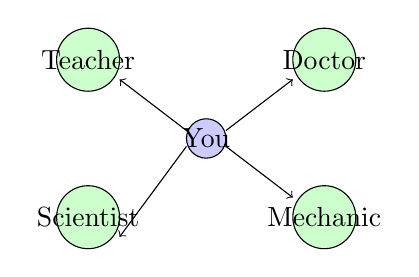
\begin{tikzpicture}[scale=0.5]
			\draw[fill=blue!20] (0,0) circle (0.5cm) node {You};
			\draw[fill=green!20] (3,2) circle (0.8cm) node {Doctor};
			\draw[fill=green!20] (3,-2) circle (0.8cm) node {Mechanic};
			\draw[fill=green!20] (-3,2) circle (0.8cm) node {Teacher};
			\draw[fill=green!20] (-3,-2) circle (0.8cm) node {Scientist};
			\draw[->] (0.5,0.2) -- (2.2,1.5);
			\draw[->] (0.5,-0.2) -- (2.2,-1.5);
			\draw[->] (-0.5,0.2) -- (-2.2,1.5);
			\draw[->] (-0.5,-0.2) -- (-2.2,-2.5);
		\end{tikzpicture}
	\end{frame}
	
	% Slide 7: The Necessity of Trust in Modern Life
	\begin{frame}
		\frametitle{The Necessity of Trust in Modern Life}
		\begin{itemize}
			\item Modern life requires constant reliance on authorities: we trust engineers who design bridges, pharmacists who fill prescriptions, and pilots who fly planes.
			\item \textbf{Epistemic dependence} refers to our necessary reliance on others for knowledge—it's not optional in complex societies.
			\item Without appeals to authority, we'd be paralyzed by the need to personally verify every claim before acting on it.
			\item The question isn't whether to trust authorities, but rather how to distinguish trustworthy authorities from unreliable ones.
		\end{itemize}
		
		\begin{alertblock}{Consider This}
			Every time you take medication, you're making an implicit argument from authority: "Medical researchers say this is safe and effective, therefore it probably is."
		\end{alertblock}
	\end{frame}
	
	% Slide 8: Ancient Medicine: When Bloodletting Was "Expert" Advice
	\begin{frame}
		\frametitle{Ancient Medicine: When Bloodletting Was "Expert" Advice}
		\begin{itemize}
			\small
			\item For over 2,000 years, bloodletting was standard medical practice, endorsed by authorities from Hippocrates to respected 19th-century physicians.
			\item \textbf{Bloodletting} involved deliberately removing blood to cure diseases, based on the theory that illness came from "bad blood" or imbalanced humors.
			\item This practice persisted not due to evidence but because of \textbf{argumentum ad antiquitatem}—the false belief that long-standing practices must be correct.
			\item George Washington likely died from excessive bloodletting in 1799, showing how even the most respected authorities can be dangerously wrong.
		\end{itemize}
		
		\begin{example}
			\scriptsize
			Medical authorities bled patients for conditions including:
			\begin{itemize}
				\item Pneumonia
				\item Fevers
				\item Back pain
				\item Mental illness
			\end{itemize}
		\end{example}
	\end{frame}
	
	% Slide 9: The Four Humors: 2,000 Years of Medical Consensus
	\begin{frame}
		\frametitle{The Four Humors: 2,000 Years of Medical Consensus}
		\begin{itemize}
			\item The \textbf{theory of the four humors} dominated medical thinking from ancient Greece through the 18th century, claiming health depended on balancing blood, phlegm, yellow bile, and black bile.
			\item This theory enjoyed near-universal \textbf{expert consensus} for millennia—virtually every medical authority from Hippocrates to Galen endorsed it.
			\item Treatments based on humoral theory included bloodletting, purging, and inducing vomiting—all aimed at "rebalancing" the body's fluids.
			\item The longevity of this false consensus shows that even widespread agreement among authorities can persist for centuries without empirical support.
		\end{itemize}
		
		\begin{block}{The Four Humors}
			\begin{tabular}{ll}
				Blood & Associated with air, spring, courage \\
				Phlegm & Associated with water, winter, calm \\
				Yellow bile & Associated with fire, summer, anger \\
				Black bile & Associated with earth, autumn, melancholy
			\end{tabular}
		\end{block}
	\end{frame}
	
	% Slide 10: Ignaz Semmelweis: When Authorities Rejected Handwashing
	\begin{frame}
		\frametitle{Ignaz Semmelweis: When Authorities Rejected Handwashing}
		\begin{itemize}
			\small
			\item In 1847, \textbf{Ignaz Semmelweis} discovered that handwashing with chlorinated lime dramatically reduced deaths from childbed fever in maternity wards.
			\item Despite clear statistical evidence—mortality rates dropped from 18\% to less than 2\%—the medical establishment rejected his findings.
			\item Authorities dismissed Semmelweis because his theory contradicted established beliefs and seemed to blame doctors for patient deaths.
			\item Semmelweis was eventually fired and suffered a mental breakdown; handwashing wasn't widely accepted until decades after his death, costing countless lives.
		\end{itemize}
		
		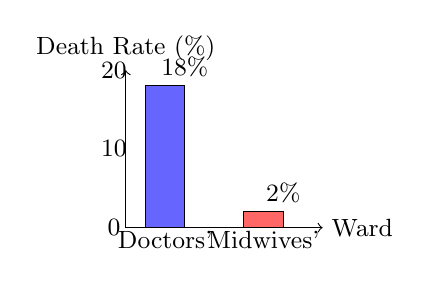
\begin{tikzpicture}[scale=0.5]
			\small
			% Axes
			\draw[->] (0,0) -- (5,0) node[right] {Ward};
			\draw[->] (0,0) -- (0,4) node[above] {Death Rate (\%)};
			
			% Bars
			\draw[fill=blue!60] (0.5,0) rectangle (1.5,3.6) node[above] {18\%};
			\draw[fill=red!60] (3,0) rectangle (4,0.4) node[above] {2\%};
			
			% Labels
			\node at (1,-0.3) {Doctors'};
			\node at (3.5,-0.3) {Midwives'};
			
			% Y-axis labels
			\node at (-0.3,0) {0};
			\node at (-0.3,2) {10};
			\node at (-0.3,4) {20};
		\end{tikzpicture}
	\end{frame}
	
	% Slide 11: The Radium Girls: When Experts Said It Was Safe
	\begin{frame}
		\frametitle{The Radium Girls: When Experts Said It Was Safe}
		\begin{itemize}
			\item In the 1920s, young women painted watch dials with radium-based paint, instructed by supervisors to lick their brushes to create fine points.
			\item Company experts and doctors assured workers that radium was safe—even beneficial—despite management knowing about radiation dangers.
			\item The \textbf{"Radium Girls"} developed severe radiation poisoning: their bones crumbled, jaws rotted away, and many died agonizing deaths.
			\item This case illustrates how \textbf{conflicts of interest} can corrupt expert testimony—company-paid doctors denied obvious connections between radium and illness.
		\end{itemize}
		
		\begin{alertblock}{Key Lesson}
			When evaluating expert claims, always consider who pays the expert and what interests they might serve.
		\end{alertblock}
	\end{frame}
	
	% Slide 12: Thalidomide: FDA Approval and Devastating Consequences
	\begin{frame}
		\frametitle{Thalidomide: FDA Approval and Devastating Consequences}
		\begin{itemize}
			\item \textbf{Thalidomide} was marketed in the late 1950s as a safe sedative for pregnant women, approved by health authorities in over 40 countries.
			\item Medical experts promoted it as "completely safe" with "no side effects"—it was even sold over-the-counter in some countries.
			\item The drug caused severe birth defects in over 10,000 children worldwide before being withdrawn in 1961-62.
			\item One FDA reviewer, Frances Kelsey, prevented U.S. approval by demanding more safety data—showing how a single skeptical authority can be right against consensus.
		\end{itemize}
		
		\begin{example}
			This tragedy led to major reforms:
			\begin{itemize}
				\item Stricter drug testing requirements
				\item Mandatory clinical trials for pregnant women
				\item Enhanced FDA regulatory powers
				\item International drug monitoring systems
			\end{itemize}
		\end{example}
	\end{frame}
	
	% Slide 13: Lobotomies: Nobel Prize-Winning Medical Malpractice
	\begin{frame}
		\frametitle{Lobotomies: Nobel Prize-Winning Medical Malpractice}
		\begin{itemize}
			\item The \textbf{prefrontal lobotomy}, a procedure that severed connections in the brain's frontal lobe, was performed on over 40,000 Americans between 1936 and 1970.
			\item António Egas Moniz won the 1949 Nobel Prize in Medicine for developing this procedure, giving it the highest possible medical authority endorsement.
			\item Patients often became emotionally blunted, childlike, or severely disabled—yet authorities promoted it as a miracle cure for mental illness.
			\item The lobotomy's acceptance shows how even Nobel Prize-level recognition doesn't guarantee a treatment is beneficial or ethical.
		\end{itemize}
		
		\begin{alertblock}{Walter Freeman's "Ice Pick" Method}
			Dr. Freeman performed over 3,500 lobotomies, including the transorbital technique—inserting an ice pick through the eye socket to damage the brain.
		\end{alertblock}
	\end{frame}
	
	\begin{frame}
		\frametitle{Authority in Modern Medicine and Science}
		\begin{itemize}
			\item As the examples in the previous slides show, medical authorities have made mistakes. This is true of all authorities (and is an inherent feature of this way of reasoning)!
			\item Modern medicine (and science) has changed in response to these problems -- though the use of \textbf{randomized control trials}, \textbf{meta-analyses} of many studies, \textbf{open data} standards and more stringent ethical guidelines on clinical trials and treatment.
			\item Since about 1930 or so, "listening to your doctor" (e.g., getting vaccines, taking antibiotics) has, on average, been good for people's health. 
			\item Debates over who is (and isn't) a medical authority have continued to rage, sometimes with disastrous results for people's health.
		\end{itemize}
		
	\end{frame}
	
	% Slide 14: Legitimate vs. Illegitimate Appeals to Authority
	\begin{frame}
		\frametitle{Legitimate vs. Illegitimate Appeals to Authority}
		\begin{itemize}
			\item A \textbf{legitimate appeal to authority} occurs when the cited expert has genuine expertise in the relevant field and represents mainstream scientific opinion.
			\item An \textbf{illegitimate appeal} (the fallacy of false authority) happens when someone lacks relevant expertise or makes claims outside their field.
			\item The difference often depends on context: a physicist discussing quantum mechanics is legitimate; the same physicist endorsing a diet plan is not.
			\item Remember that even legitimate appeals are defeasible—new evidence can overturn expert consensus.
		\end{itemize}
		
		\begin{table}
			\centering
			\scriptsize
			\begin{tabular}{|p{4cm}|p{4cm}|}
				\hline
				\textbf{Legitimate} & \textbf{Illegitimate} \\
				\hline
				Cardiologist on heart disease & Celebrity on vaccines \\
				Climate scientist on global warming & Politician on evolution \\
				Historian on ancient Rome & Engineer on psychology \\
				Pharmacist on drug interactions & YouTuber on cancer cures \\
				\hline
			\end{tabular}
		\end{table}
	\end{frame}
	
	
	
	% Slide 15: Direct Expertise vs. Adjacent Fields
	\begin{frame}
		\frametitle{Direct Expertise vs. Adjacent Fields}
		\begin{itemize}
			\item \textbf{Direct expertise} means having specialized training and experience in the exact area under discussion.
			\item \textbf{Adjacent field expertise} occurs when someone knowledgeable in a related but distinct area comments outside their specialty.
			\item The closer the fields, the more weight we might give to adjacent expertise—but critical differences can make such appeals unreliable.
			\item Many false appeals to authority exploit our difficulty in distinguishing genuine expertise from adjacent or irrelevant credentials.
		\end{itemize}
		
		\begin{example}
			A neurosurgeon (brain surgery expert) commenting on:
			\begin{itemize}
				\item Brain tumor treatment → Direct expertise 
				\item General neurology → Adjacent field (somewhat reliable)
				\item Psychiatry → More distant field (less reliable)
				\item Nutrition → Unrelated field (not reliable)
			\end{itemize}
		\end{example}
	\end{frame}
	
	% Slide 16: Individual Experts vs. Institutional Authority
	\begin{frame}
		\frametitle{Individual Experts vs. Institutional Authority}
		\begin{itemize}
			\item \textbf{Individual experts} offer personal judgment based on their training and experience, but may have biases or make errors.
			\item \textbf{Institutional authorities} like the CDC, WHO, or medical associations represent collective expertise and undergo peer review processes.
			\item Institutions can provide more reliable guidance through systematic review processes, but can also suffer from groupthink or bureaucratic inertia.
			\item The strongest appeals to authority often combine both: individual experts whose views align with institutional consensus.
		\end{itemize}
		
		\begin{block}{Hierarchy of Medical Authority}
			\begin{enumerate}
				\item Systematic reviews and meta-analyses
				\item Professional medical associations' guidelines
				\item Peer-reviewed research by multiple teams
				\item Individual expert opinions
				\item Single studies or anecdotal evidence
			\end{enumerate}
		\end{block}
	\end{frame}
	
	% Slide 17: Cultural Authority vs. Scientific Authority
	\begin{frame}
		\frametitle{Cultural Authority vs. Scientific Authority}
		\begin{itemize}
			\item \textbf{Cultural authorities} derive their credibility from tradition, religious position, or social status within a community.
			\item \textbf{Scientific authorities} base their expertise on empirical research, peer review, and the scientific method.
			\item These two types of authority can conflict, especially in areas like medicine where traditional practices meet modern science.
			\item Understanding this distinction helps explain why some communities reject vaccines or climate science despite overwhelming scientific consensus.
		\end{itemize}
		
		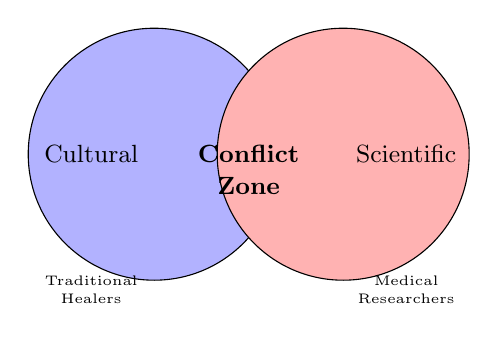
\begin{tikzpicture}[scale=0.8]
			% Two circles with partial overlap
			\draw[fill=blue!30] (-1.5,0) circle (2cm);
			\draw[fill=red!30] (1.5,0) circle (2cm);
			\node at (-2.5,0) {\small Cultural};
			\node at (2.5,0) {\small Scientific};
			\node at (0,0) {\small \textbf{Conflict}};
			\node at (0,-0.5) {\small \textbf{Zone}};
			% Examples
			\node at (-2.5,-2) {\tiny Traditional};
			\node at (-2.5,-2.3) {\tiny Healers};
			\node at (2.5,-2) {\tiny Medical};
			\node at (2.5,-2.3) {\tiny Researchers};
		\end{tikzpicture}
	\end{frame}
	
	% Slide 18: Dr. Oz and TV Medical Advice: Entertainment or Expertise?
	\begin{frame}
		\frametitle{Dr. Oz and TV Medical Advice: Entertainment or Expertise?}
		\begin{itemize}
			\item Dr. Mehmet Oz began as a respected cardiac surgeon but transformed into a television personality offering daily medical advice.
			\item A 2014 study found that \textbf{40\% of Dr. Oz's medical recommendations contradicted available scientific evidence} or lacked any supporting research.
			\item The \textbf{"Dr. Oz Effect"} demonstrates how media platforms can amplify questionable medical claims by mixing entertainment with expertise.
			\item His case illustrates the danger when legitimate credentials are used to promote products and treatments outside one's expertise or without scientific support.
		\end{itemize}
		
		\begin{alertblock}{Senate Hearing (2014)}
			Dr. Oz was called before Congress to explain his promotion of "miracle" weight loss products that research showed were ineffective.
		\end{alertblock}
	\end{frame}
	
	% Slide 19: Social Media Health Influencers: The New "Authorities"
	\begin{frame}
		\frametitle{Social Media Health Influencers: The New "Authorities"}
		\begin{itemize}
			\item \textbf{Health influencers} on Instagram, TikTok, and YouTube often present themselves as authorities despite lacking medical training or credentials.
			\item Many followers treat these influencers as experts based solely on personal transformation stories, attractive presentations, or follower counts.
			\item The \textbf{parasocial relationships} formed online can make followers trust influencers more than their own doctors.
			\item This phenomenon bypasses traditional gatekeeping mechanisms like peer review, licensing boards, and professional accountability.
		\end{itemize}
		
		\begin{example}
			\scriptsize
			Common Red Flags in Health Influencer Content:
			\begin{itemize}
				\item "Doctors don't want you to know..."
				\item Selling expensive supplements or programs
				\item Claiming one solution fixes everything
				\item Rejecting all mainstream medicine
			\end{itemize}
		\end{example}
	\end{frame}
	
	% Slide 20: Celebrity Endorsements: When Fame Becomes "Expertise"
	\begin{frame}
		\frametitle{Celebrity Endorsements: When Fame Becomes "Expertise"}
		\begin{itemize}
			\item \textbf{Celebrity medical advocacy} occurs when famous individuals promote health claims based on personal experience rather than scientific evidence.
			\item The \textbf{halo effect} causes people to assume that success in one area (acting, sports) translates to credibility in health matters.
			\item Celebrities often share compelling personal stories that feel more relatable than statistics, making their false authority particularly persuasive.
			\item This becomes dangerous when celebrities contradict medical consensus on issues like vaccines, cancer treatment, or mental health.
		\end{itemize}
		
		\begin{block}{Case Study: Jenny McCarthy}
			\scriptsize
			\begin{tabular}{p{4cm}p{6cm}}
				\textbf{Background:} & Actress and model \\
				\textbf{Claimed Authority:} & "Mother's intuition" about vaccines \\
				\textbf{Impact:} & Influenced vaccine hesitancy movement \\
				\textbf{Problem:} & No medical or scientific training
			\end{tabular}
		\end{block}
	\end{frame}
	
	% Slide 20a: Financial Gurus: When "Experts" Sell Hope
	\begin{frame}
		\frametitle{Financial Gurus: When "Experts" Sell Hope}
		\begin{itemize}
			\item \textbf{Financial influencers} often present themselves as authorities based on personal wealth stories rather than financial expertise or fiduciary responsibility.
			\item The \textbf{survivorship bias} means we hear from those who got lucky, not the thousands who failed using identical strategies.
			\item Many "gurus" profit from selling courses and seminars, not from the investment strategies they promote—a clear conflict of interest.
			\item Legitimate financial authorities have certifications (CFP, CFA), fiduciary duties, and don't promise unrealistic returns.
		\end{itemize}
		
		\begin{alertblock}{Red Flags in Financial Advice}
			\begin{itemize}
				\item "I made millions with this ONE trick..."
				\item "Guaranteed 50\% returns!"
				\item Expensive courses teaching "secrets"
				\item No mention of risk or downside
			\end{itemize}
		\end{alertblock}
	\end{frame}
	
	% Slide 20b: Crime Statistics: How Politicians and Media Misuse Authority
	\begin{frame}
		\frametitle{Crime Statistics: How Politicians and Media Misuse Authority}
		\begin{itemize}
			\item Politicians and media outlets often cite \textbf{crime statistics} selectively, presenting themselves as authorities on public safety trends.
			\item The \textbf{availability heuristic} makes vivid individual cases seem representative, even when statistics show crime decreasing overall.
			\item Different authorities (FBI, local police, advocacy groups) use different methodologies, enabling cherry-picking of supportive data.
			\item Understanding base rates, per capita calculations, and trend lines is crucial for evaluating claims about crime.
		\end{itemize}
		
		\begin{example}
			Same Data, Different Claims:
			\begin{itemize}
				\item "Murders increased 30\%!" (True: from 10 to 13 in small town)
				\item "City is safer than ever!" (Also true: overall crime down 15\%)
				\item "Violence is exploding!" (Misleading: one category up, most down)
			\end{itemize}
		\end{example}
	\end{frame}
	
	
	% Slide 20e: Parenting Advice: When Everyone Knows Best
	\begin{frame}
		\frametitle{Parenting Advice: When Everyone Knows Best}
		\begin{itemize}
			\item \textbf{Parenting authorities} range from pediatricians and child psychologists to mommy bloggers and family members—all claiming expertise.
			\item The \textbf{naturalistic fallacy} leads many to assume traditional or "natural" parenting methods are automatically superior to evidence-based approaches.
			\item Social media creates echo chambers where dangerous practices (like avoiding vaccines) seem normal because "everyone" in the group agrees.
			\item Legitimate child development expertise requires understanding research methods, not just having successfully raised children.
		\end{itemize}
		
		\begin{alertblock}{The "Mom Group" Problem}
			Online parenting groups often elevate personal anecdotes over pediatric consensus, creating alternative "authorities" that contradict medical advice on sleep, feeding, and safety.
		\end{alertblock}
	\end{frame}
	
	% Slide 21: AI Medical Chatbots: Can Algorithms Be Authorities?
	\begin{frame}
		\frametitle{AI Medical Chatbots: Can Algorithms Be Authorities?}
		\begin{itemize}
			\item \textbf{AI medical systems} like ChatGPT, Claude, and specialized medical chatbots are increasingly consulted for health information and advice.
			\item These systems can access vast medical databases but lack clinical experience, medical training, and the ability to physically examine patients.
			\item The \textbf{automation bias} leads people to trust AI recommendations simply because they come from a computer, assuming objectivity.
			\item AI presents unique challenges: it can sound authoritative while "hallucinating" false information or missing critical context about individual cases.
		\end{itemize}
		
		\begin{alertblock}{Key Limitation}
			AI systems explicitly state they cannot provide medical advice, yet users often treat their responses as authoritative medical guidance.
		\end{alertblock}
	\end{frame}
	
	% Slide 22: WebMD Syndrome: Self-Diagnosis in the Information Age
	\begin{frame}
		\frametitle{WebMD Syndrome: Self-Diagnosis in the Information Age}
		\begin{itemize}
			\item \textbf{"WebMD Syndrome"} or \textbf{cyberchondria} occurs when people self-diagnose serious conditions based on internet searches of common symptoms.
			\item Search engines and medical websites become de facto authorities, but they lack the clinical judgment to weigh symptom probability and context.
			\item The availability of medical information creates an illusion of expertise—people feel qualified to challenge their doctors' diagnoses.
			\item This phenomenon shows how access to information without proper training can lead to misuse of legitimate medical resources.
		\end{itemize}
		
		\begin{example}
			\scriptsize
			Common WebMD Progression:
			\begin{enumerate}
				\item Symptom: "Headache"
				\item Search results include: Brain tumor, aneurysm, meningitis
				\item Anxiety increases symptoms
				\item Demands unnecessary tests from doctor
			\end{enumerate}
		\end{example}
	\end{frame}
	
	% Slide 23: Anti-Vaccine Movements: Competing Claims to Authority
	\begin{frame}
		\frametitle{Anti-Vaccine Movements: Competing Claims to Authority}
		\begin{itemize}
			\item Modern \textbf{anti-vaccine movements} create alternative authority structures that compete with mainstream medical consensus.
			\item These movements often cite discredited studies, minority medical opinions, or non-experts presented as whistleblowers against "Big Pharma."
			\item The \textbf{false balance} in media coverage gives equal weight to scientific consensus and fringe theories, confusing public understanding.
			\item Social media echo chambers allow these alternative authorities to seem more credible through repetition and community reinforcement.
		\end{itemize}
		
		\begin{block}{Competing Authority Claims}
			\begin{tabular}{|l|l|}
				\hline
				\textbf{Scientific Consensus} & \textbf{Anti-Vaccine Claims} \\
				\hline
				Thousands of studies & One retracted study \\
				Medical associations & "Brave" individual doctors \\
				Peer review process & Parent testimonials \\
				Global health data & Anecdotal evidence \\
				\hline
			\end{tabular}
		\end{block}
	\end{frame}
	
	% Slide 24: What Makes Someone a Genuine Expert?
	\begin{frame}
		\frametitle{What Makes Someone a Genuine Expert?}
		\begin{itemize}
			\item \textbf{Genuine expertise} requires formal education, practical experience, and ongoing engagement with current research in a specific field.
			\item True experts acknowledge uncertainty, cite sources, and change positions when presented with new evidence.
			\item \textbf{Metacognitive awareness}—knowing the limits of one's knowledge—distinguishes real experts from false authorities.
			\item Genuine experts participate in professional communities where their work undergoes scrutiny and peer review.
		\end{itemize}
		
		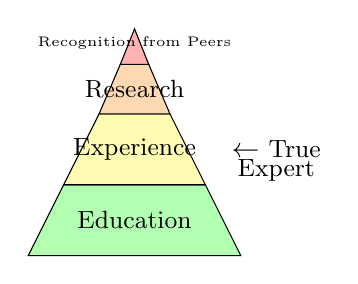
\begin{tikzpicture}[scale=0.9]
			% Pyramid of expertise
			\draw[fill=green!30] (0,0) -- (3,0) -- (2.5,1) -- (0.5,1) -- cycle;
			\draw[fill=yellow!30] (0.5,1) -- (2.5,1) -- (2,2) -- (1,2) -- cycle;
			\draw[fill=orange!30] (1,2) -- (2,2) -- (1.7,2.7) -- (1.3,2.7) -- cycle;
			\draw[fill=red!30] (1.3,2.7) -- (1.7,2.7) -- (1.5,3.2) -- cycle;
			
			\node at (1.5,0.5) {\small Education};
			\node at (1.5,1.5) {\small Experience};
			\node at (1.5,2.35) {\small Research};
			\node at (1.5,3.0) {\tiny Recognition from Peers};
			\node at (3.5,1.5) {$\leftarrow$ \small True};
			\node at (3.5,1.2) {\small Expert};
		\end{tikzpicture}
	\end{frame}
	
	% Slide 25: Credentials, Experience, and Peer Recognition
	\begin{frame}
		\frametitle{Credentials, Experience, and Peer Recognition}
		\begin{itemize}
			\item \textbf{Credentials} include degrees, licenses, and certifications from accredited institutions—but these alone don't guarantee current expertise.
			\item \textbf{Relevant experience} means actually working in the field, treating patients, conducting research, or solving real problems over time.
			\item \textbf{Peer recognition} appears through citations, invited lectures, leadership positions, and awards from professional communities.
			\item The strongest authorities combine all three: proper credentials, extensive experience, and recognition from other experts in their field.
		\end{itemize}
		
		\begin{table}
			\centering
			\small
			\begin{tabular}{|l|c|c|c|}
				\hline
				\textbf{Example} & \textbf{Credentials} & \textbf{Experience} & \textbf{Peer Recognition} \\
				\hline
				New MD graduate & Yes & No & No \\
				Veteran doctor & Yes & Yes & Varies \\
				Nobel laureate & Yes & Yes & Yes \\
				"TV doctor" & Yes & Limited & No \\
				\hline
			\end{tabular}
		\end{table}
	\end{frame}
	
	% Slide 26: Understanding Scientific Consensus
	\begin{frame}
		\frametitle{Understanding Scientific Consensus}
		\begin{itemize}
			\item \textbf{Scientific consensus} emerges when the vast majority of experts in a field agree based on accumulated evidence.
			\item Consensus doesn't mean unanimous agreement—there are almost always some dissenters, but we must evaluate their credibility and motivations.
			\item Strong consensus develops through multiple independent studies, replication of results, and rigorous peer review over time.
			\item The strength of consensus varies: climate change (97\%+ agreement) represents stronger consensus than optimal nutrition guidelines (more debate).
		\end{itemize}
		
		\begin{block}{Markers of Strong Consensus}
			\scriptsize
			\begin{itemize}
				\item Multiple professional organizations agree
				\item Reproduced across different countries/labs
				\item Decades of consistent findings
				\item Dissenters can't publish in best peer-reviewed journals
				\item Predictions based on consensus prove accurate
			\end{itemize}
		\end{block}
	\end{frame}
	
	% Slide 27: When Experts Disagree: Navigating Conflicting Opinions
	\begin{frame}
		\frametitle{When Experts Disagree: Navigating Conflicting Opinions}
		\begin{itemize}
			\item Expert disagreement is normal in emerging fields, complex questions, or areas with limited data.
			\item When experts disagree, examine whether it's about \textbf{fundamental facts} (rare) or \textbf{interpretation and application} (common).
			\item Consider the proportion of experts on each side—is it 50/50 or 95/5? The latter suggests examining minority views skeptically.
			\item In cases of genuine expert disagreement, reasonable people should acknowledge uncertainty rather than choosing sides prematurely.
		\end{itemize}
		
		\begin{example}
			COVID-19 mask recommendations in early 2020:
			\begin{itemize}
				\item Initial disagreement due to limited data
				\item Experts revised positions as evidence emerged
				\item Consensus developed around indoor masking
				\item Legitimate debate continued on outdoor requirements
			\end{itemize}
		\end{example}
	\end{frame}
	
	% Slide 28: The Role of Peer Review and Replication
	\begin{frame}
		\frametitle{The Role of Peer Review and Replication}
		\begin{itemize}
			\item \textbf{Peer review} acts as quality control, where other experts evaluate research methods, logic, and conclusions before publication.
			\item \textbf{Replication} means other researchers repeat experiments to verify results—crucial for establishing reliable knowledge.
			\item The \textbf{replication crisis} revealed that many published findings, especially in psychology and medicine, couldn't be reproduced.
			\item These mechanisms aren't perfect but provide essential checks against individual bias, fraud, and honest errors.
		\end{itemize}
		
		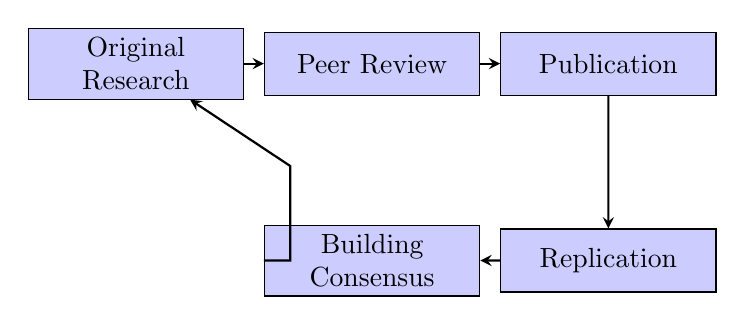
\begin{tikzpicture}[scale=0.8, node distance=2cm]
			% Define styles
			\tikzstyle{process} = [rectangle, draw, fill=blue!20, text width=2.5cm, text centered, minimum height=0.8cm]
			\tikzstyle{arrow} = [thick,->,>=stealth]
			
			% Nodes
			\node[process] (research) {Original Research};
			\node[process] (peer) [right of=research, xshift=1cm] {Peer Review};
			\node[process] (publish) [right of=peer, xshift=1cm] {Publication};
			\node[process] (replicate) [below of=publish, yshift=-0.5cm] {Replication};
			\node[process] (consensus) [left of=replicate, xshift=-1cm] {Building Consensus};
			
			% Arrows
			\draw[arrow] (research) -- (peer);
			\draw[arrow] (peer) -- (publish);
			\draw[arrow] (publish) -- (replicate);
			\draw[arrow] (replicate) -- (consensus);
			\draw[arrow] (consensus) -- ++(-1.3,0) -- ++(0,1.5) -- (research);
		\end{tikzpicture}
	\end{frame}
	
	% Slide 29: Identifying Conflicts of Interest
	\begin{frame}
		\frametitle{Identifying Conflicts of Interest}
		\begin{itemize}
			\item A \textbf{conflict of interest} occurs when an expert has financial, personal, or professional incentives that might bias their judgment.
			\item Common conflicts include funding from pharmaceutical companies, personal investments in recommended treatments, or career advancement tied to specific outcomes.
			\item Conflicts don't automatically invalidate expertise, but they require extra scrutiny—especially when recommendations benefit the expert financially.
			\item Reputable experts disclose conflicts openly; be suspicious of those who hide financial relationships or claim complete objectivity.
		\end{itemize}
		
		\begin{alertblock}{Red Flag Examples}
			\begin{itemize}
				\item Doctor selling their own supplement brand
				\item Researcher funded solely by industry
				\item Expert witness paid by one side
				\item Study author owns patents on findings
			\end{itemize}
		\end{alertblock}
	\end{frame}
	
	% Slide 30: False Authority: When Expertise Doesn't Transfer
	\begin{frame}
		\frametitle{False Authority: When Expertise Doesn't Transfer}
		\begin{itemize}
			\item The \textbf{false authority fallacy} occurs when someone's expertise in one area is wrongly assumed to apply in unrelated fields.
			\item This fallacy exploits our tendency to view intelligence and competence as general rather than domain-specific traits.
			\item Even brilliant experts become laypeople outside their specialties—a Nobel physicist has no special insight into nutrition or politics.
			\item Media often amplifies this fallacy by seeking opinions from famous experts on topics beyond their expertise.
		\end{itemize}
		
		\begin{example}
			Classic Examples of Non-Transferable Expertise:
			\begin{itemize}
				\item Linus Pauling (Chemistry Nobel) promoting vitamin C megadoses
				\item Dr. Ben Carson (neurosurgeon) on archaeological theories
				\item Richard Dawkins (biologist) on philosophy of religion
			\end{itemize}
		\end{example}
	\end{frame}
	
	% Slide 31: Cherry-Picking Experts: Finding the One Who Agrees
	\begin{frame}
		\frametitle{Cherry-Picking Experts: Finding the One Who Agrees}
		\begin{itemize}
			\item \textbf{Cherry-picking experts} means searching until you find the rare authority who supports your predetermined position.
			\item With thousands of experts worldwide, you can almost always find someone with credentials who holds any position, no matter how fringe.
			\item This tactic creates false equivalence—presenting one dissenting expert as equal to hundreds who disagree.
			\item Media often enables cherry-picking through "both sides" coverage that elevates minority positions to seem equally valid.
		\end{itemize}
		
		\begin{block}{The 97\% Problem}
			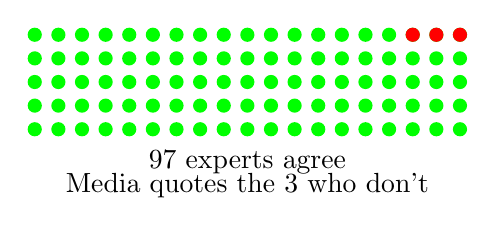
\begin{tikzpicture}[scale=0.6]
				% Draw 97 green dots and 3 red dots
				\foreach \x in {0,0.5,1,1.5,2,2.5,3,3.5,4,4.5,5,5.5,6,6.5,7,7.5,8,8.5,9}
				\foreach \y in {0,0.5,1,1.5,2}
				{\fill[green] (\x,\y) circle (0.15cm);}
				% Make 3 dots red
				\fill[red] (9,2) circle (0.15cm);
				\fill[red] (8.5,2) circle (0.15cm);
				\fill[red] (8,2) circle (0.15cm);
				\node at (4.5,-0.7) {97 experts agree};
				\node at (4.5,-1.2) {Media quotes the 3 who don't};
			\end{tikzpicture}
		\end{block}
	\end{frame}
	
	% Slide 32: Outdated Authority: When Knowledge Evolves
	\begin{frame}
		\frametitle{Outdated Authority: When Knowledge Evolves}
		\begin{itemize}
			\item \textbf{Outdated authority} occurs when we rely on experts whose knowledge hasn't kept pace with new discoveries and evolving consensus.
			\item Medical knowledge has a "half-life"—studies suggest about 50\% of medical knowledge becomes outdated within 10-15 years.
			\item Retired experts may cling to theories from their training, unaware of subsequent research that disproved their beliefs.
			\item This problem intensifies in rapidly advancing fields like genetics, neuroscience, and technology-related health issues.
		\end{itemize}
		
		\begin{table}
			\centering
			\begin{tabular}{|l|l|l|}
				\hline
				\textbf{Field} & \textbf{Old Authority} & \textbf{Current Understanding} \\
				\hline
				Nutrition & Fats are always bad & Some fats essential \\
				Psychology & Refrigerator mothers & Autism is genetic \\
				Ulcers & Caused by stress & H. pylori bacteria \\
				Brain & No new neurons & Neurogenesis occurs \\
				\hline
			\end{tabular}
		\end{table}
	\end{frame}
	
	% Slide 33: Anonymous Authority: "Studies Show" and "Experts Say"
	\begin{frame}
		\frametitle{Anonymous Authority: "Studies Show" and "Experts Say"}
		\begin{itemize}
			\item \textbf{Anonymous authority} appeals cite unnamed experts or unspecified research to create an illusion of scientific support.
			\item Phrases like "studies show," "scientists say," or "research proves" without citations are red flags for weak or fabricated authority.
			\item Legitimate experts name their sources, cite specific studies, and provide enough information for verification.
			\item This tactic is especially common in advertising, social media health claims, and politically motivated arguments.
		\end{itemize}
		
		\begin{alertblock}{Warning Phrases}
			\begin{itemize}
				\item "9 out of 10 doctors recommend..." (Which doctors? Selected how?)
				\item "Research has shown..." (What research? By whom?)
				\item "Experts agree..." (Which experts? In what field?)
				\item "Clinical studies prove..." (Published where? Peer reviewed?)
			\end{itemize}
		\end{alertblock}
	\end{frame}
	
	% Slide 34: Questions to Ask Before Accepting Expert Opinion
	\begin{frame}
		\frametitle{Questions to Ask Before Accepting Expert Opinion}
		\begin{itemize}
			\item Before accepting an expert's claim, systematically evaluate both the expert and their specific assertion.
			\item These questions help distinguish legitimate authority from false or misleading appeals.
			\item The more important the decision, the more rigorously you should apply these criteria.
			\item Remember: even good experts can be wrong, but following this process reduces your risk of being misled.
		\end{itemize}
		
		\begin{block}{Essential Questions Checklist}
			\scriptsize
			\begin{enumerate}
				\item Is this person actually an expert in THIS specific topic?
				\item What are their relevant credentials and experience?
				\item Do other experts in the field agree or disagree?
				\item Are there any conflicts of interest?
				\item Is the claim within scientific consensus?
				\item How recent is their expertise?
				\item Can I verify their sources?
			\end{enumerate}
		\end{block}
	\end{frame}
	
	% Slide 35: Finding and Evaluating Primary Sources
	\begin{frame}
		\frametitle{Finding and Evaluating Primary Sources}
		\begin{itemize}
			\item \textbf{Primary sources} in medicine include peer-reviewed research papers, clinical trial data, and systematic reviews—not news articles about them.
			\item Learning to read scientific abstracts helps you verify whether experts accurately represent research findings.
			\item Tools like PubMed, Google Scholar, and Cochrane Reviews provide access to legitimate medical literature.
			\item When experts disagree, examining primary sources reveals whether disagreement stems from different interpretations of the same data.
		\end{itemize}
		
		\begin{example}
			\scriptsize
			Hierarchy of Medical Evidence:
			\begin{enumerate}
				\item Systematic reviews and meta-analyses
				\item Randomized controlled trials (RCTs)
				\item Cohort studies
				\item Case-control studies
				\item Expert opinion and case reports
			\end{enumerate}
			Always prefer sources higher on this list!
		\end{example}
	\end{frame}
	
	% Slide 36: Building a Network of Trusted Sources
	\begin{frame}
		\frametitle{Building a Network of Trusted Sources}
		\begin{itemize}
			\item Develop a personal network of reliable sources for different domains—specific experts, institutions, and publications you've learned to trust.
			\item Verify new claims by checking whether your trusted sources have addressed them and what positions they take.
			\item Update your network as you discover errors—no source is infallible, but some consistently prove more reliable than others.
			\item Building information literacy is a lifelong process that protects against misinformation while keeping you open to new knowledge.
		\end{itemize}
		
		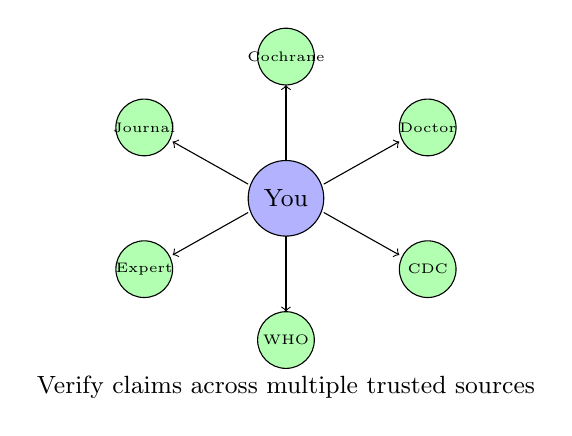
\begin{tikzpicture}[scale=0.6]
			% Center node
			\draw[fill=blue!30] (0,0) circle (0.8cm) node {\small You};
			
			% Trusted sources around
			\draw[fill=green!30] (3,1.5) circle (0.6cm) node {\tiny Doctor};
			\draw[fill=green!30] (3,-1.5) circle (0.6cm) node {\tiny CDC};
			\draw[fill=green!30] (-3,1.5) circle (0.6cm) node {\tiny Journal};
			\draw[fill=green!30] (-3,-1.5) circle (0.6cm) node {\tiny Expert};
			\draw[fill=green!30] (0,3) circle (0.6cm) node {\tiny Cochrane};
			\draw[fill=green!30] (0,-3) circle (0.6cm) node {\tiny WHO};
			
			% Connections
			\draw[->] (0.8,0.3) -- (2.4,1.2);
			\draw[->] (0.8,-0.3) -- (2.4,-1.2);
			\draw[->] (-0.8,0.3) -- (-2.4,1.2);
			\draw[->] (-0.8,-0.3) -- (-2.4,-1.2);
			\draw[->] (0,0.8) -- (0,2.4);
			\draw[->] (0,-0.8) -- (0,-2.4);
			
			\node at (0,-4) {\small Verify claims across multiple trusted sources};
		\end{tikzpicture}
	\end{frame}
	
\end{document}